\chapter{Architektura systemu i reprodukowalność eksperymentów}
\label{chap:architektura-systemu-reprodukowalnosc}

W niniejszym rozdziale przedstawiono warstwę inżynieryjną i techniczną projektu. Badania oparte na uczeniu maszynowym wymagają nie tylko oceny skuteczności predykcyjnej, opisanej w rozdziale~\ref{chap:wyniki-interpretacja-modeli}, lecz także zapewnienia odtwarzalności (ang. \emph{reproducibility}). Zgodnie z dobrymi praktykami oprogramowania naukowego, na przykład postulatami \emph{The Turing Way} \cite{TuringWay2025}, rzetelne badanie powinno być możliwe do niezależnego odtworzenia na podstawie dostarczonego kodu i danych. W tym celu wdrożono uporządkowaną architekturę systemu, skonteneryzowane środowisko Docker, zautomatyzowane skrypty wykonawcze oraz zestaw testów.

\section{Środowisko wdrożeniowe i konteneryzacja (Docker)}
\label{sec:srodowisko-wdrozeniowe-konteneryzacja}

Podstawą reprodukowalności wdrożonego rozwiązania jest skonteneryzowanie go przy użyciu technologii Docker \cite{Merkel2014}. Zamiast opierać się na lokalnych środowiskach programistycznych, które mogą różnić się konfiguracją i zależnościami, cały system analityczny i aplikacyjny został umieszczony w izolowanym obrazie.

\subsection{Uzasadnienie złożoności systemu (Dlaczego MLOps?)}
\label{subsec:uzasadnienie-zlozonosci-systemu-mlops}

Na pierwszy rzut oka do wytrenowania modelu uczenia maszynowego mógłby wystarczyć pojedynczy skrypt w Pythonie. Potrzeba zastosowania bardziej rozbudowanej architektury Docker, izolowanych potoków i środowisk testowych wynika jednak bezpośrednio z charakteru problemu badawczego.

Praca na 160 tysiącach epizodów zwierząt obejmujących 10 lat działalności schroniska wiąże się z istotnym ryzykiem wycieku danych (ang. \emph{data leakage}). W nieustrukturyzowanym kodzie łatwo o sytuację, w której podczas transformacji danych przypadkowo uwzględniona zostanie informacja z przyszłości, na przykład powód eutanazji jako predyktor, mimo że model ma działać już na etapie przyjęcia zwierzęcia. Dodatkowym problemem jest zjawisko ,,cichej degradacji'' (ang. \emph{silent failure}). W przypadku błędnie podanych danych model nie musi wygenerować technicznego błędu, takiego jak \texttt{Exception}, lecz może bez widocznego ostrzeżenia zwrócić nieprawidłową predykcję ryzyka. Z tego powodu uporządkowana infrastruktura MLOps była ważna dla zapewnienia bezstronności, audytowalności i kontroli jakości wygenerowanych rezultatów, a nie tylko dla uzyskania wysokich metryk.

\subsection{Architektura serwisów (Docker Compose)}
\label{subsec:architektura-serwisow-docker-compose}

Zastosowano narzędzie Docker Compose (\texttt{docker-compose.yml}), które definiuje architekturę systemu jako zbiór odseparowanych kontenerów, czyli serwisów, korzystających ze wspólnych zasobów. Taka struktura pozwala uruchomić wybraną warstwę systemu za pomocą jednej komendy. W ramach architektury zdefiniowano następujące serwisy operacyjne:

\begin{lstlisting}[caption={Kluczowe definicje serwisów wyizolowane w architekturze docker-compose.yml},label={lst:docker-compose-services}]
services:
  dashboard:
    build: .
    ports: ["8501:8501"]
    volumes: [./models:/app/models]
  pipeline-full:
    build: .
    command: python scripts/run_full_pipeline.py
    volumes: [./data:/app/data, ./reports:/app/reports]
  test:
    build: .
    command: python -m pytest tests/ -v
\end{lstlisting}

Wszystkie te serwisy współdzielą na poziomie kontenerów zmapowane wolumeny pamięci, czyli katalogi \texttt{data/}, \texttt{models/}, \texttt{reports/} i \texttt{logs/}. Umożliwia to przepływ wytworzonych artefaktów między poszczególnymi warstwami bez powielania danych. Istotne jest także odseparowanie zapisu od konsumpcji: \texttt{pipeline-full} zapisuje artefakty do katalogu \texttt{reports/}, natomiast \texttt{dashboard} korzysta z modeli zapisanych w katalogu \texttt{models/}. Relacje między głównymi serwisami a udostępnianymi katalogami zilustrowano na rysunku~\ref{fig:docker_compose_arch}.

\begin{figure}[htbp]
\centering
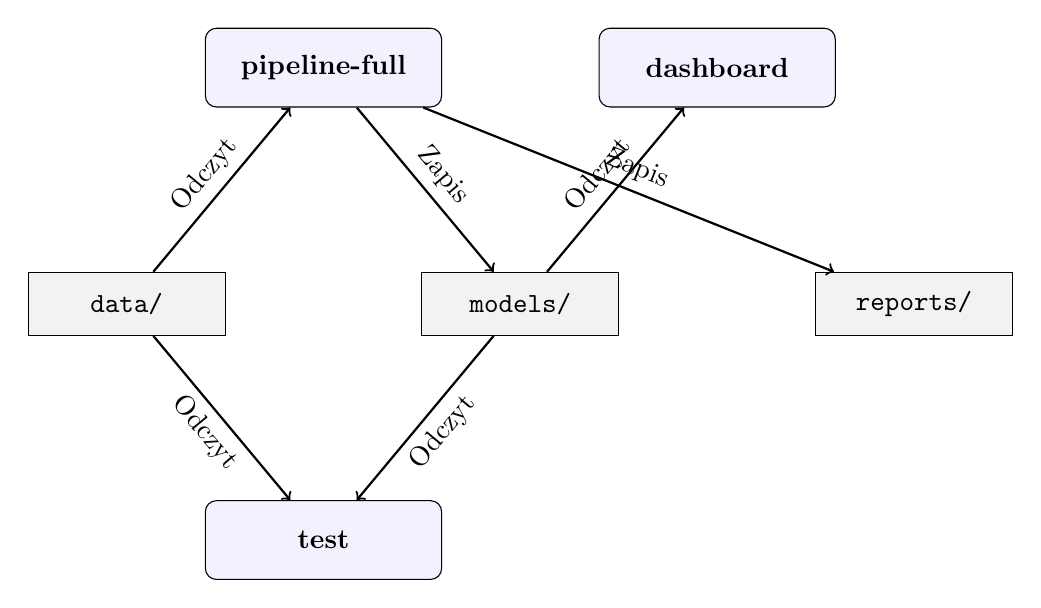
\begin{tikzpicture}[
  service/.style={draw, rectangle, rounded corners, minimum width=3cm, minimum height=1cm, align=center, fill=blue!5},
  volume/.style={draw, rectangle, minimum width=2.5cm, minimum height=0.8cm, align=center, fill=gray!10},
  arrow/.style={->, thick}
]

% Volumes at y=0
\node[volume] (data) at (0, 0) {\texttt{data/}};
\node[volume] (models) at (5, 0) {\texttt{models/}};
\node[volume] (reports) at (10, 0) {\texttt{reports/}};

% Services at y=3
\node[service] (pipeline) at (2.5, 3) {\textbf{pipeline-full}};
\node[service] (dashboard) at (7.5, 3) {\textbf{dashboard}};

% Service at y=-3
\node[service] (test) at (2.5, -3) {\textbf{test}};

% Pipeline Connections
\draw[arrow] (data) -- (pipeline) node[midway, sloped, above] {Odczyt};
\draw[arrow] (pipeline) -- (models) node[midway, sloped, above] {Zapis};
\draw[arrow] (pipeline) -- (reports) node[midway, sloped, above] {Zapis};

% Dashboard Connections
\draw[arrow] (models) -- (dashboard) node[midway, sloped, above] {Odczyt};

% Test Connections
\draw[arrow] (data) -- (test) node[midway, sloped, below] {Odczyt};
\draw[arrow] (models) -- (test) node[midway, sloped, below] {Odczyt};

\end{tikzpicture}
\caption{Architektura serwisów Docker Compose i udostępniane wolumeny pamięci}
\label{fig:docker_compose_arch}
\end{figure}

\section{Architektura \emph{Artifact-First} i separacja warstw}
\label{sec:artifact-first-separacja-warstw}

Dzięki skonteneryzowaniu różnych ról systemu możliwe było zastosowanie podejścia \emph{Artifact-First}. Oznacza ono ścisłe rozdzielenie zasobochłonnego procesu uczenia modeli od lekkiej warstwy prezentacyjnej, czyli aplikacji dla użytkownika końcowego.

Decyzja ta wynika z praktycznych ograniczeń środowiska docelowego. Typowe placówki ratownictwa zwierząt nie dysponują infrastrukturą serwerową wyposażoną w akceleratory graficzne (GPU), które mogą być potrzebne do efektywnego trenowania wybranych modeli. Dodatkowo interaktywne retrenowanie modelu po wprowadzeniu każdego nowego zwierzęcia, czyli tzw. uczenie online, wiązałoby się z ryzykiem operacyjnym. Błędnie wprowadzony rekord mógłby szybko pogorszyć jakość działania całego systemu.

\begin{itemize}
    \item \textbf{Warstwa eksperymentalna (Jupyter):} przeznaczona dla \emph{data scientistów} do testowania hipotez.
    \item \textbf{Warstwa treningowa (Pipeline):} z uwagi na duży wolumen danych, obejmujący ponad 160 tys. epizodów, operacje te zajmują znaczny czas. Wyniki uruchomienia kontenera \texttt{pipeline-full} są ,,zamrażane'' w formie statycznych artefaktów: wyuczonych modeli w formacie \texttt{.joblib}, tabel wyników w formacie \texttt{.csv} oraz wygenerowanych wykresów \texttt{.png}.
    \item \textbf{Warstwa konsumpcyjna (Dashboard):} aplikacja demonstracyjna, opisana w rozdziale~\ref{chap:aplikacja-demonstracyjna-prezentacja-wynikow}, nie posiada uprawnień do modyfikacji algorytmów. Jej rola ogranicza się do ładowania do pamięci RAM gotowych modeli zapisanych na dysku.
\end{itemize}

Takie podejście obniża wymagania sprzętowe po stronie serwera aplikacji i wspiera niezmienność decyzji algorytmicznych. Pracownik schroniska otrzymuje predykcję z modelu wcześniej przetestowanego, a nie z modelu zmienionego najnowszymi danymi.

\section{Organizacja kodu i modułowość}
\label{sec:organizacja-kodu-modulowosc}

Projekt ustrukturyzowano jako standardowy pakiet języka Python zarządzany przez \texttt{pyproject.toml}. Struktura repozytorium (listing~\ref{lst:dir-tree}) odpowiada podziałowi kompetencji:

\begin{lstlisting}[language=bash, caption={Drzewo katalogów głównego projektu}, label={lst:dir-tree}]
austin-analysis/
|-- docker-compose.yml
|-- pyproject.toml
|-- src/
|   `-- aac_adoption/
|       |-- data/
|       |-- features/
|       |-- models/
|       `-- reporting/
|-- scripts/
|   `-- run_full_pipeline.py
|-- tests/
|-- notebooks/
|-- models/
`-- reports/
\end{lstlisting}

\begin{enumerate}
    \item \texttt{src/aac\_adoption/} -- główny kod źródłowy biblioteki, podzielony na domeny: \texttt{data} (przetwarzanie epizodów), \texttt{features} (rejestr cech), \texttt{models} (uczenie i ewaluacja) oraz \texttt{reporting} (agregacja wyników).
    \item \texttt{scripts/} -- narzędzia wykonawcze (CLI), np. skrypt \texttt{run\_full\_pipeline.py}.
    \item \texttt{tests/} -- zestaw zautomatyzowanych testów jednostkowych i integracyjnych uruchamianych z kontenera testowego.
    \item \texttt{notebooks/} -- notatniki Jupyter służące analizie odkrywczej.
\end{enumerate}

\section{Automatyzacja potoku (Pipeline) a notatniki Jupyter}
\label{sec:automatyzacja-potoku-notatniki-jupyter}

W uczeniu maszynowym częstym problemem jest ,,ukryty dług techniczny'' (ang. \emph{hidden technical debt}) \cite{Sculley2015}. Modele budowane wyłącznie przez sekwencyjne uruchamianie komórek w notatnikach Jupyter mogą stać się trudne do odtworzenia.

Dlatego w niniejszej architekturze Jupyter (\texttt{notebooks/}) służy wyłącznie do badania i rozwoju (R\&D). Gdy dana logika okazuje się skuteczna, jest przenoszona do produkcyjnego kodu źródłowego w \texttt{src/}. Ostateczne trenowanie modeli realizowane jest przez w pełni skryptowy, centralny potok wywoływany w kontenerze \texttt{pipeline-full}:

\begin{lstlisting}[caption={Uruchomienie pełnego potoku eksperymentalnego},label={lst:pipeline-full-command}]
docker-compose up pipeline-full
\end{lstlisting}

\subsection{Fazy zautomatyzowanego potoku i Data Provenance}
\label{subsec:fazy-potoku-data-provenance}

Komenda ta zamyka proces badawczy w deterministycznych ramach, uruchamiając sekwencyjnie 18 zdefiniowanych kroków widocznych w skrypcie \texttt{run\_full\_pipeline.py}. Proces ten można podzielić na następujące makrofazy:

\begin{enumerate}
    \item \textbf{Zarządzanie danymi:} automatyczne pobranie surowych danych, jeśli ich brakuje, czyszczenie oraz budowa ujednoliconego zbioru (\texttt{build\_dataset}).
    \item \textbf{Modelowanie:} trening modeli bazowych, strojenie hiperparametrów algorytmów drzewiastych oraz kalibracja klasyfikatorów.
    \item \textbf{Diagnostyka i wyjaśnialność:} generowanie wykresów diagnostycznych i przeliczanie wartości SHAP dla całego zbioru.
    \item \textbf{Raportowanie:} automatyczne zapisywanie artefaktów, czyli tabel i wykresów, bezpośrednio do katalogu \texttt{reports/}.
\end{enumerate}

\begin{figure}[htbp]
\centering

\includegraphics[width=0.92\textwidth]{../reports/figures/recency_strategy_comparison.png}
\caption{Porównanie strategii ewaluacji chronologicznej zastosowanej w potoku eksperymentalnym. Dane z lat 2013--2021 posłużyły do uczenia modeli, lata 2022--2023 do walidacji i doboru progu decyzyjnego, a lata 2024--2025 stanowią jednorazowy zbiór testowy. Podejście to odwzorowuje warunki rzeczywistego wdrożenia, w którym model musi generalizować na dane z przyszłości.}
\label{fig:recency-strategy}
\end{figure}

Szczególną uwagę w potoku poświęcono koncepcji \textbf{Data Provenance}, czyli proweniencji danych, oraz precyzyjnemu wersjonowaniu eksperymentów. Wersjonowanie kodu zapewnia system Git, a powiązanie konkretnej wersji kodu z odpowiednimi artefaktami realizowane jest przez autorski mechanizm pokwitowań uruchomień (ang.\ \emph{run receipts}). Każdy krok potoku wywołuje funkcję \texttt{write\_producer\_receipt()}, zapisującą do katalogu \texttt{reports/run\_receipts/} osobny plik JSON dokumentujący identyfikator uruchomienia, skrót SHA komitu Git, listę artefaktów wejściowych i wyjściowych, czas wykonania oraz status zakończenia. Integracja z narzędziem DVC (Data Version Control)~\cite{Kuprieiev2024} stanowi planowany kierunek dalszego rozwoju systemu~\cite{Kreuzberger2023}.

Po poprawnym zakończeniu 18 kroków modelowania potok generuje plik \texttt{run\_receipt.json}. Pełni on funkcję kompleksowego zapisu technicznego z przebiegu eksperymentu, dokumentując:
\begin{itemize}
    \item dokładny znacznik czasu (timestamp) rozpoczęcia i zakończenia procedur,
    \item skrót SHA komitu Git, precyzyjnie identyfikujący wersję kodu źródłowego,
    \item pełną listę wszystkich wykonanych z powodzeniem faz (od czyszczenia danych, przez inżynierię cech, strojenie hiperparametrów, aż po ocenę końcową),
    \item podsumowanie ewentualnych ostrzeżeń lub pominiętych kroków kalibracji.
\end{itemize}
Dzięki temu plikowi można bezbłędnie zidentyfikować, w jakich warunkach oraz na jakich danych trenujących powstały wyeksportowane modele.

\section{Rygor testowy i audyty danych}
\label{sec:rygor-testowy-audyty-danych}

Złożoność przetwarzania danych weryfikowano na każdym etapie za pomocą zautomatyzowanych zestawów testów, uruchamianych w ramach komendy \texttt{docker-compose up test}. Środowisko testowe pokrywa szereg krytycznych aspektów niezawodności, przede wszystkim: obronę przed wyciekiem danych informujących o przyszłości (ang. \emph{data leakage}), integralność strukturalną tabel bazowych (\emph{data integrity}) oraz spójność przejścia surowych danych przez cały zintegrowany potok (\emph{pipeline tests}). System zwraca jednoznaczne logi dokumentujące poprawność architektury:

\begin{lstlisting}[caption={Fragment wydruku środowiska testowego dokumentujący pomyślne zakończenie audytu wycieku danych (leakage audit)},label={lst:test-output-leakage-audit}]
============================= test session starts ==============================
collected 34 items

tests/test_leakage_audit.py::test_audit_leakage_columns_risk_levels  PASSED
tests/test_leakage_audit.py::test_no_leakage_columns_in_dataset      PASSED
tests/test_leakage_audit.py::test_no_future_columns_in_dataset       PASSED
tests/test_leakage_audit.py::test_all_prohibited_columns_rejected    PASSED
tests/test_split.py::test_chronological_split_dates                  PASSED
tests/test_calibration_chronology.py::test_calibration_uses_val_data PASSED
...
============================== 34 passed in 18.2s ==============================
\end{lstlisting}

Wszystkim niedeterministycznym operacjom algorytmicznym w kodzie przypisano stałe ziarno losowości (\texttt{RANDOM\_STATE = 42}). Nie zastępuje ono chronologicznego podziału danych opisanego w sekcji~\ref{sec:przygotowanie-danych-podzial}, lecz stabilizuje elementy losowe obecne w procedurach uczenia i oceny modeli:

\begin{lstlisting}[language=Python,caption={Przykład utrzymania stałego ziarna losowości w modelowaniu},label={lst:random-state-example}]
RANDOM_STATE = 42

classifier = HistGradientBoostingClassifier(random_state=RANDOM_STATE)
regressor = CatBoostRegressor(random_seed=RANDOM_STATE, verbose=False)
\end{lstlisting}

Poprawne uruchomienie całego środowiska Docker --- od potoku treningowego po warstwę prezentacyjną --- potwierdzono praktycznie. Rysunek~\ref{fig:streamlit-launch-ch6} przedstawia stronę startową aplikacji demonstracyjnej uruchomionej w kontenerze \texttt{dashboard}.

\begin{figure}[htbp]
\centering

\includegraphics[width=0.90\textwidth]{../reports/figures/streamlit_ui_tab0_full.png}
\caption{Strona główna aplikacji demonstracyjnej (Streamlit) działającej w kontenerze \texttt{dashboard} po pomyślnym zakończeniu potoku \texttt{pipeline-full}. Widoczne zakładki odpowiadają modułom funkcjonalnym opisanym w rozdziale~7.}
\label{fig:streamlit-launch-ch6}
\end{figure}

W połączeniu z powtarzalną architekturą Docker wspiera to odtwarzalność potoku analitycznego na innej maszynie serwerowej. Celem takiej organizacji jest uzyskanie tych samych tabel wyników oraz wykresów przy ponownym uruchomieniu eksperymentu, z zastrzeżeniem możliwych minimalnych różnic numerycznych wynikających z wersji bibliotek, architektury sprzętowej lub ustawień wielowątkowości. Tak rozumiana reprodukowalność odpowiada kryteriom audytowalności prac naukowych.